\newpage
\subsection{Sensor Package Design}
The sensors, the micro controller unit and the additional electronics are all combined in the sensor package. Throughout testing there has been revisions on this sensor package.\\

In the Preliminary Research Report it was stated that the project would make use out of \gls{3D} designs. As it turns out that the sensor package didn't require any unique shapes, it made better sense to edit existing enclosures, like project boxes. Throughout the project, components were acquired through  Shopee \cite{shopee} and local electronic markets like the Nhat Tao Market. \cite{nhattao}

\subsubsection{Revision 1}
The initial idea was to the components in one plastic enclosure. A project box was acquired and holes were drilled out at the side of the box to make mounts for the the turbidity, acidity, and conductivity sensors.

\begin{figure}[h]
\centering
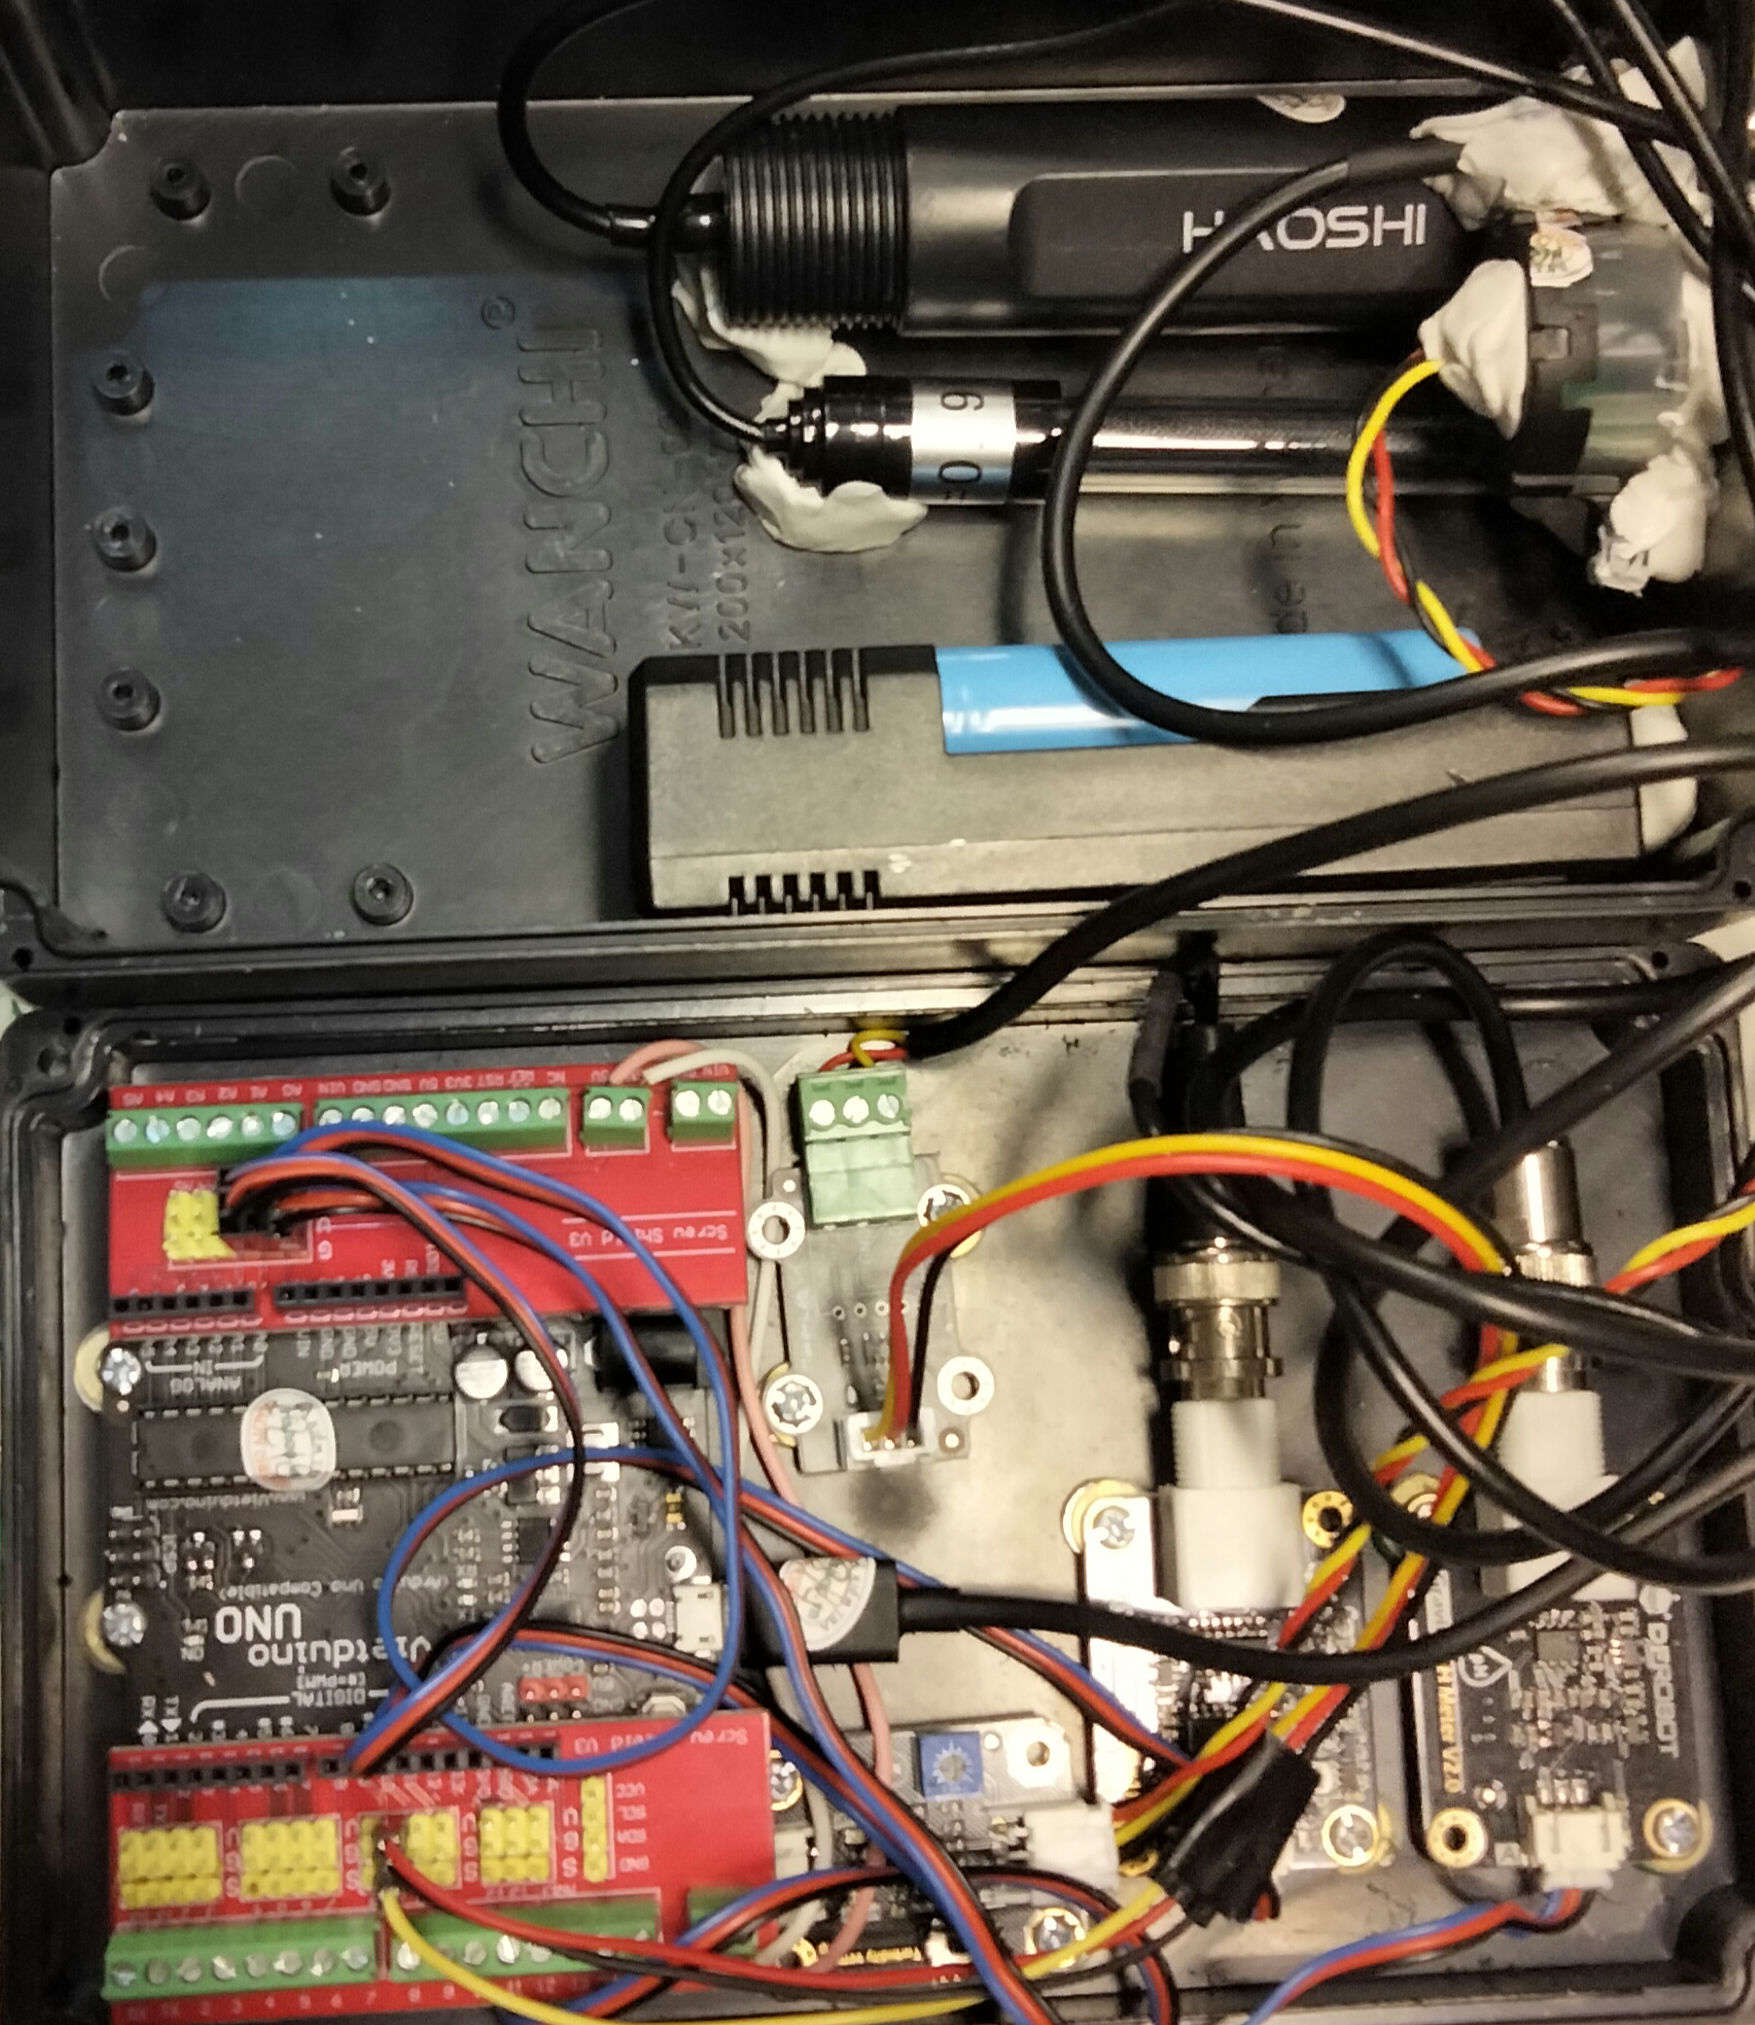
\includegraphics[scale=0.1]{070_design/package/51_rev1.jpg}
\caption{Inside of the first revision [own picture]}
\end{figure}

The bottom of the box has screw holes drilled out for mounting the \gls{PCB}s in the case. To prevent water from coming into the enclosure, O-rings are used along with sticky tack. Rubber inserts were used to close down the box. After some preliminary testing, it turned out that some water still leaked into the enclosure while fully submerged.
\newpage
\subsubsection{Revision 2}
On the second revision, a different approach was taken. The sensitive non-waterproof \gls{PCB}s were covered by a two-part epoxy, so that even if water would come into the enclosure, it would not be likely to short any circuits.\\

The \gls{PCB}s are mounted on a metal holed sheet covered with conductive tape. This way, the entire waterproof enclosure could be replaced easily in the future without dismounting any \gls{PCB}s. A swivel is used to lead the cables waterproof outside the enclosure. A battery bank is placed underneath the \gls{PCB}s for powering the electronics.

\begin{figure}[h]
  \centering
  \begin{minipage}[b]{0.4\textwidth}
    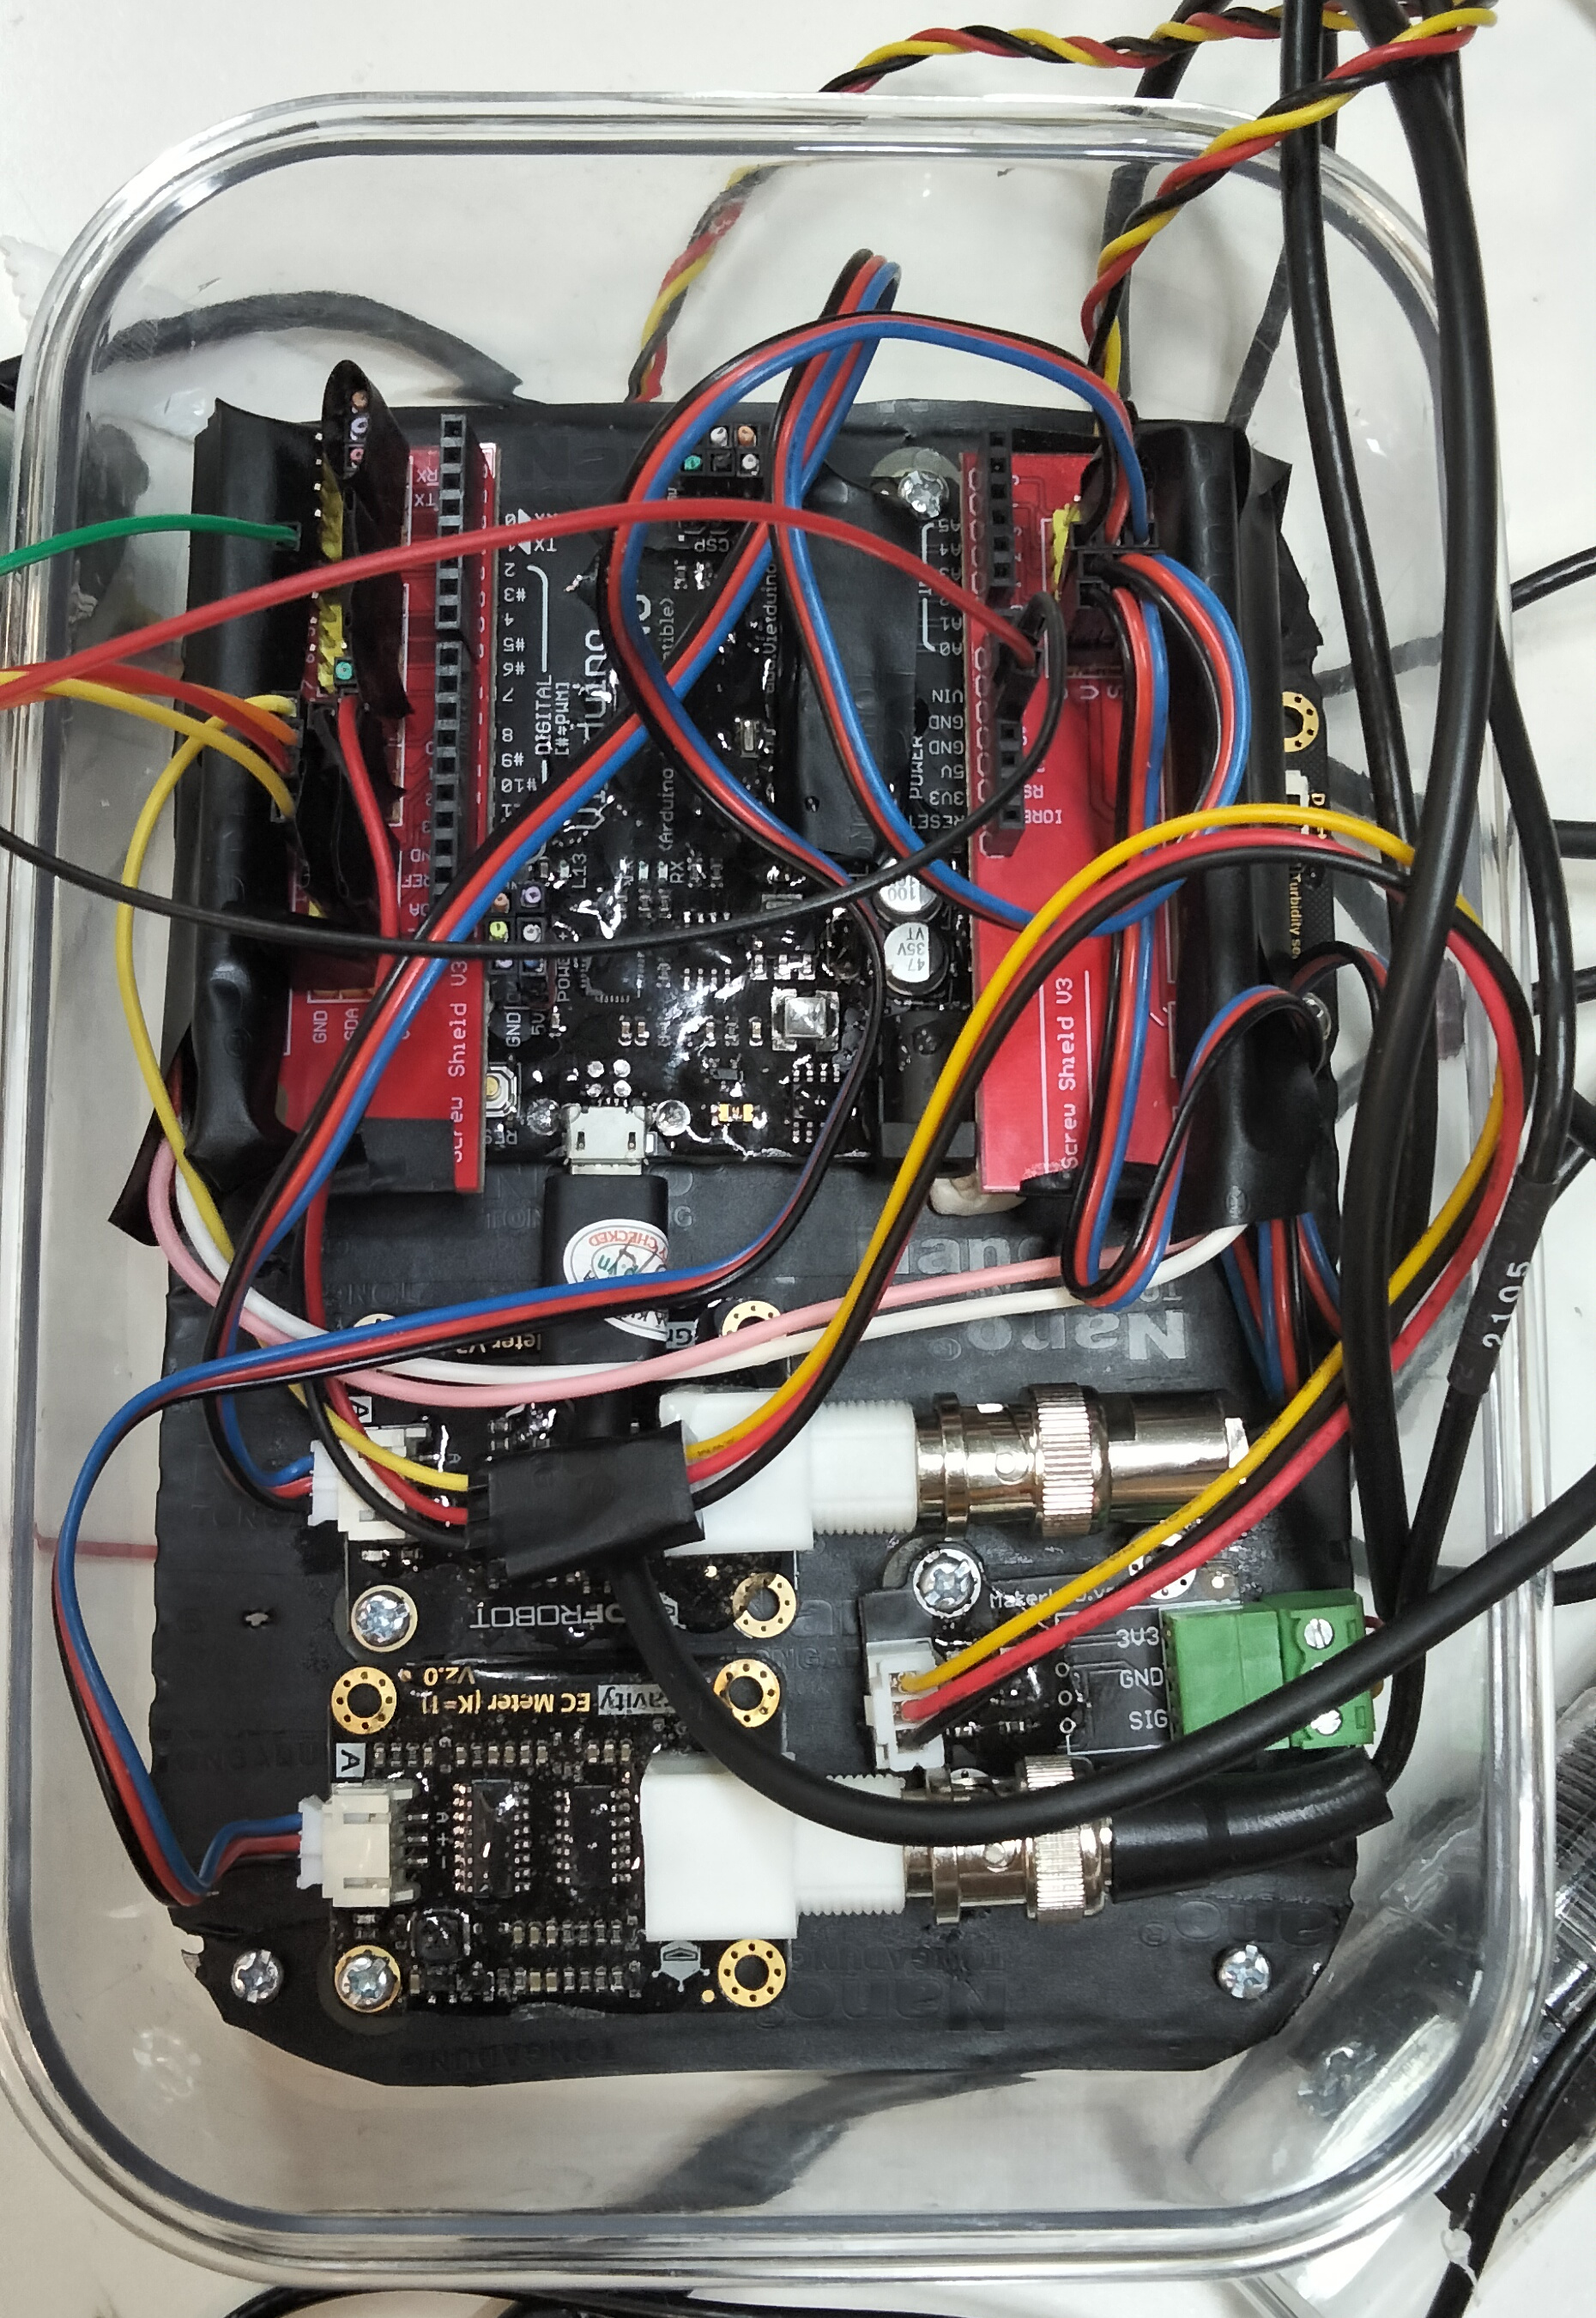
\includegraphics[width=\textwidth]{070_design/package/52_rev2.jpg}
    \caption{Inside of the second revision [own picture]}
  \end{minipage}
  \hfill
  \begin{minipage}[b]{0.5\textwidth}
    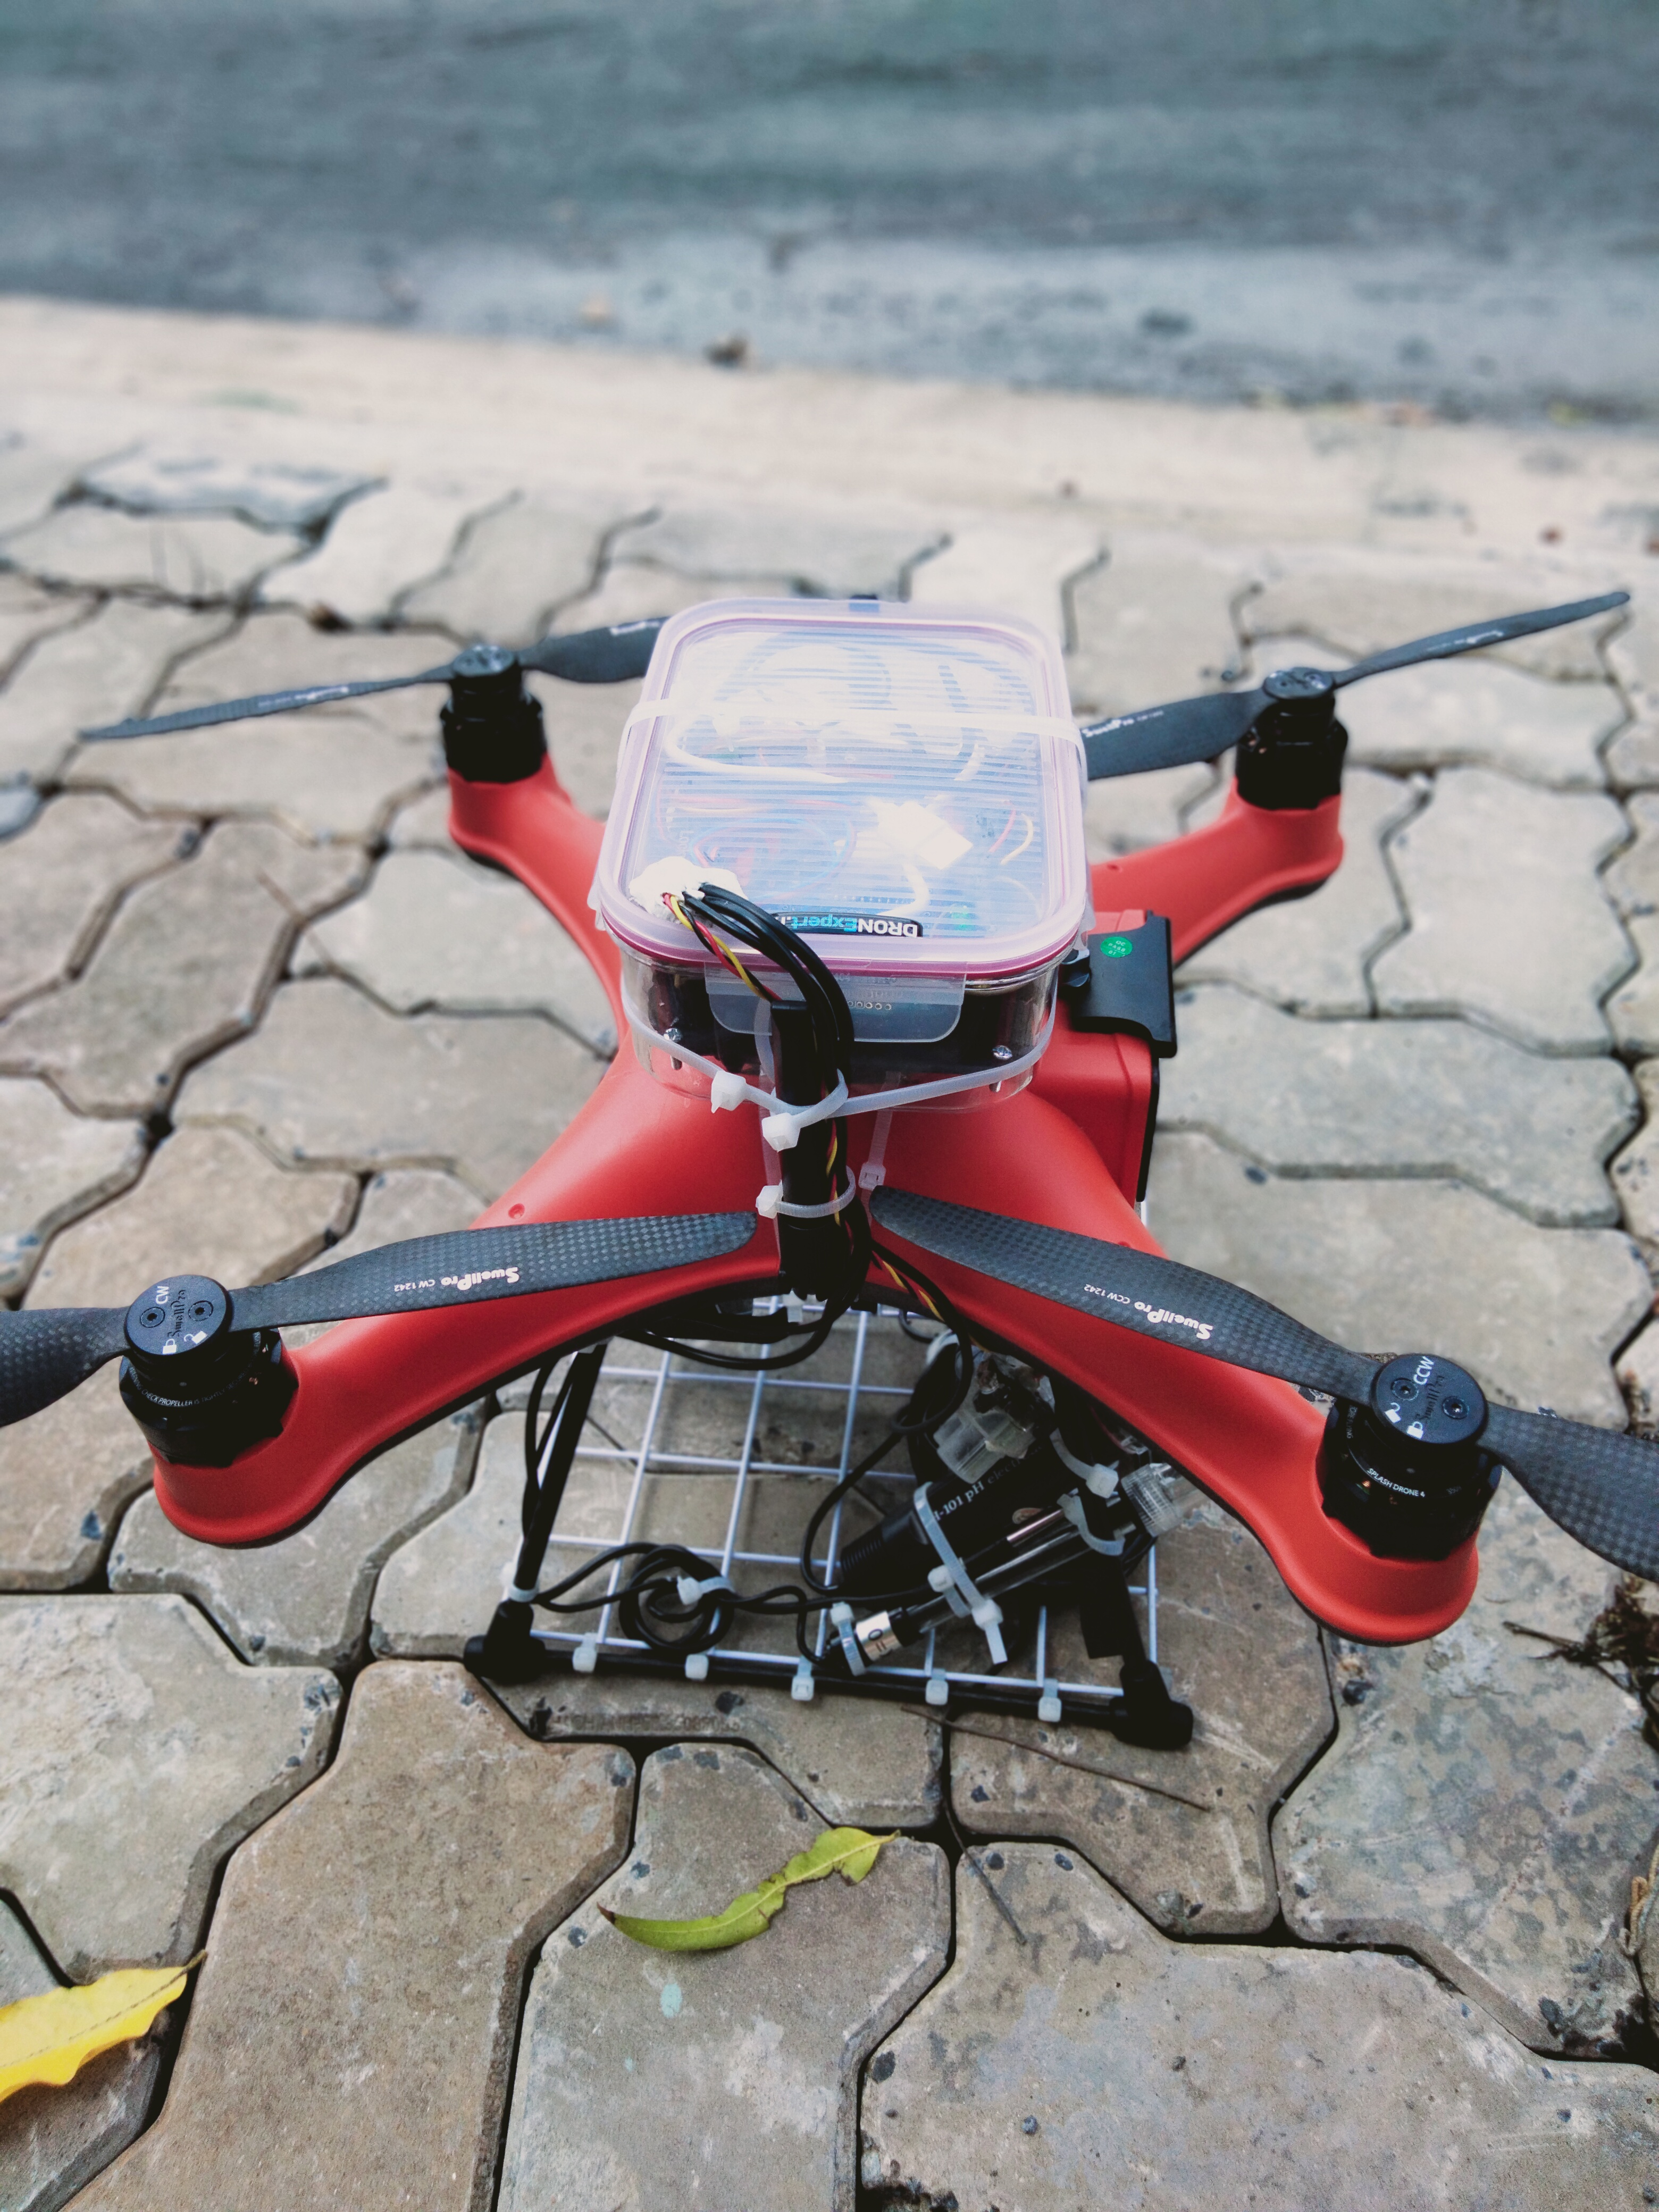
\includegraphics[width=\textwidth]{070_design/package/53_mount.jpg}
    \caption{Full view of the drone [own picture]}
  \end{minipage}
\end{figure}

The sensor probes are placed outside the enclosure on a rack underneath the drone to be fully submerged in the water, while the enclosure is placed on top of the drone above the water. The enclosure is slightly heightened so that the propellers of the drone can still move freely.\\

Throughout the drone, cable ties are used to fasten the enclosure, sensors and the rack. This is a very convenient and simple solution, as it allows one to quickly make changes to the design as the project goes forward, without investing a lot of time in a \gls{CAD} application. 

\newpage
\subsubsection{Secchi Disk}
To determine the turbidity, a secchi disk is used. This disk was made from an used 30\gls{cm} record. Tape was used to make the black and white sides. An eye bolt was used to make a hole for the rope to attach. The secchi disk is attached to the middle of the bottom grid of the drone.

\begin{figure}[h]
\centering
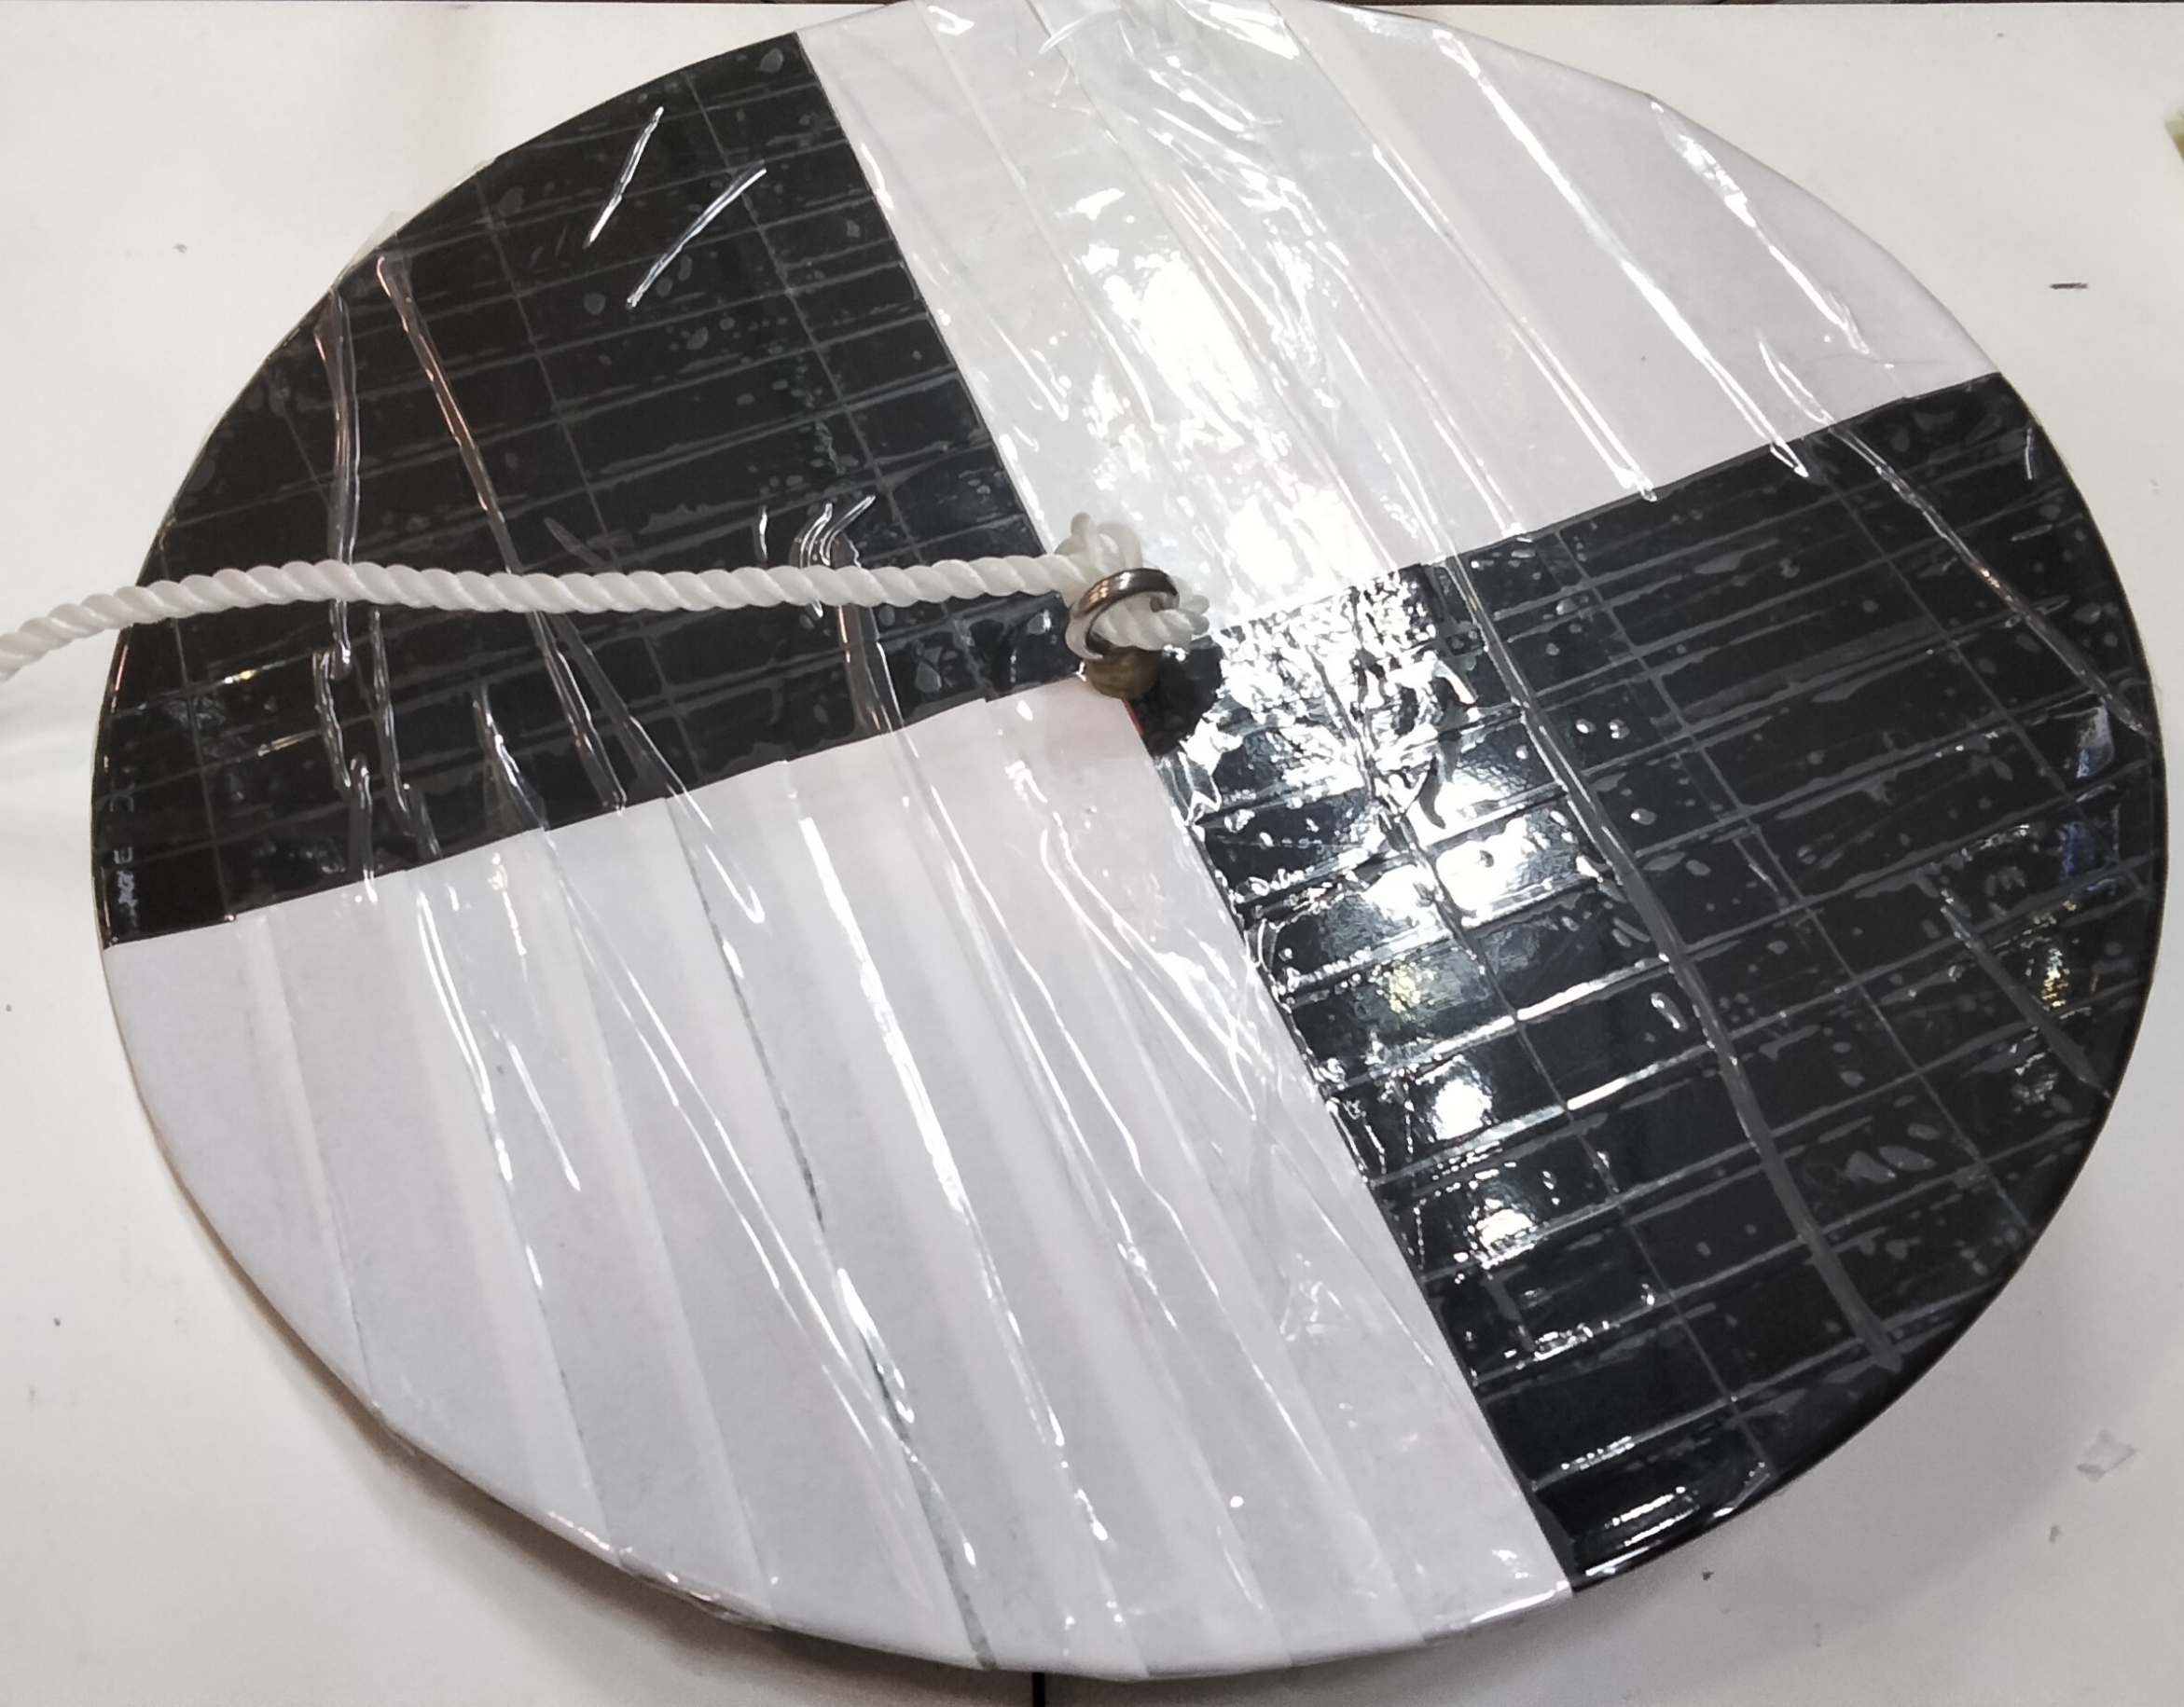
\includegraphics[scale=0.1]{070_design/package/54_secchi.jpg}
\caption{\gls{DIY} Secchi Disk [own picture]}
\end{figure}

A layer of transparent packing tape was used to cover the secchi disk to protect the colored tape. As seen in the photo, this introduces a lot of glare combined with the lighting. This may pose an issue when taking pictures.\\

Upon initial testing, it turned out that the buoyancy of the disk was too great for it to be sinking in the water. 1.2\gls{kg} weight to the disk was added by modifying and attaching a defective car ventilator to the bottom of the disk.

\begin{figure}[h]
\centering
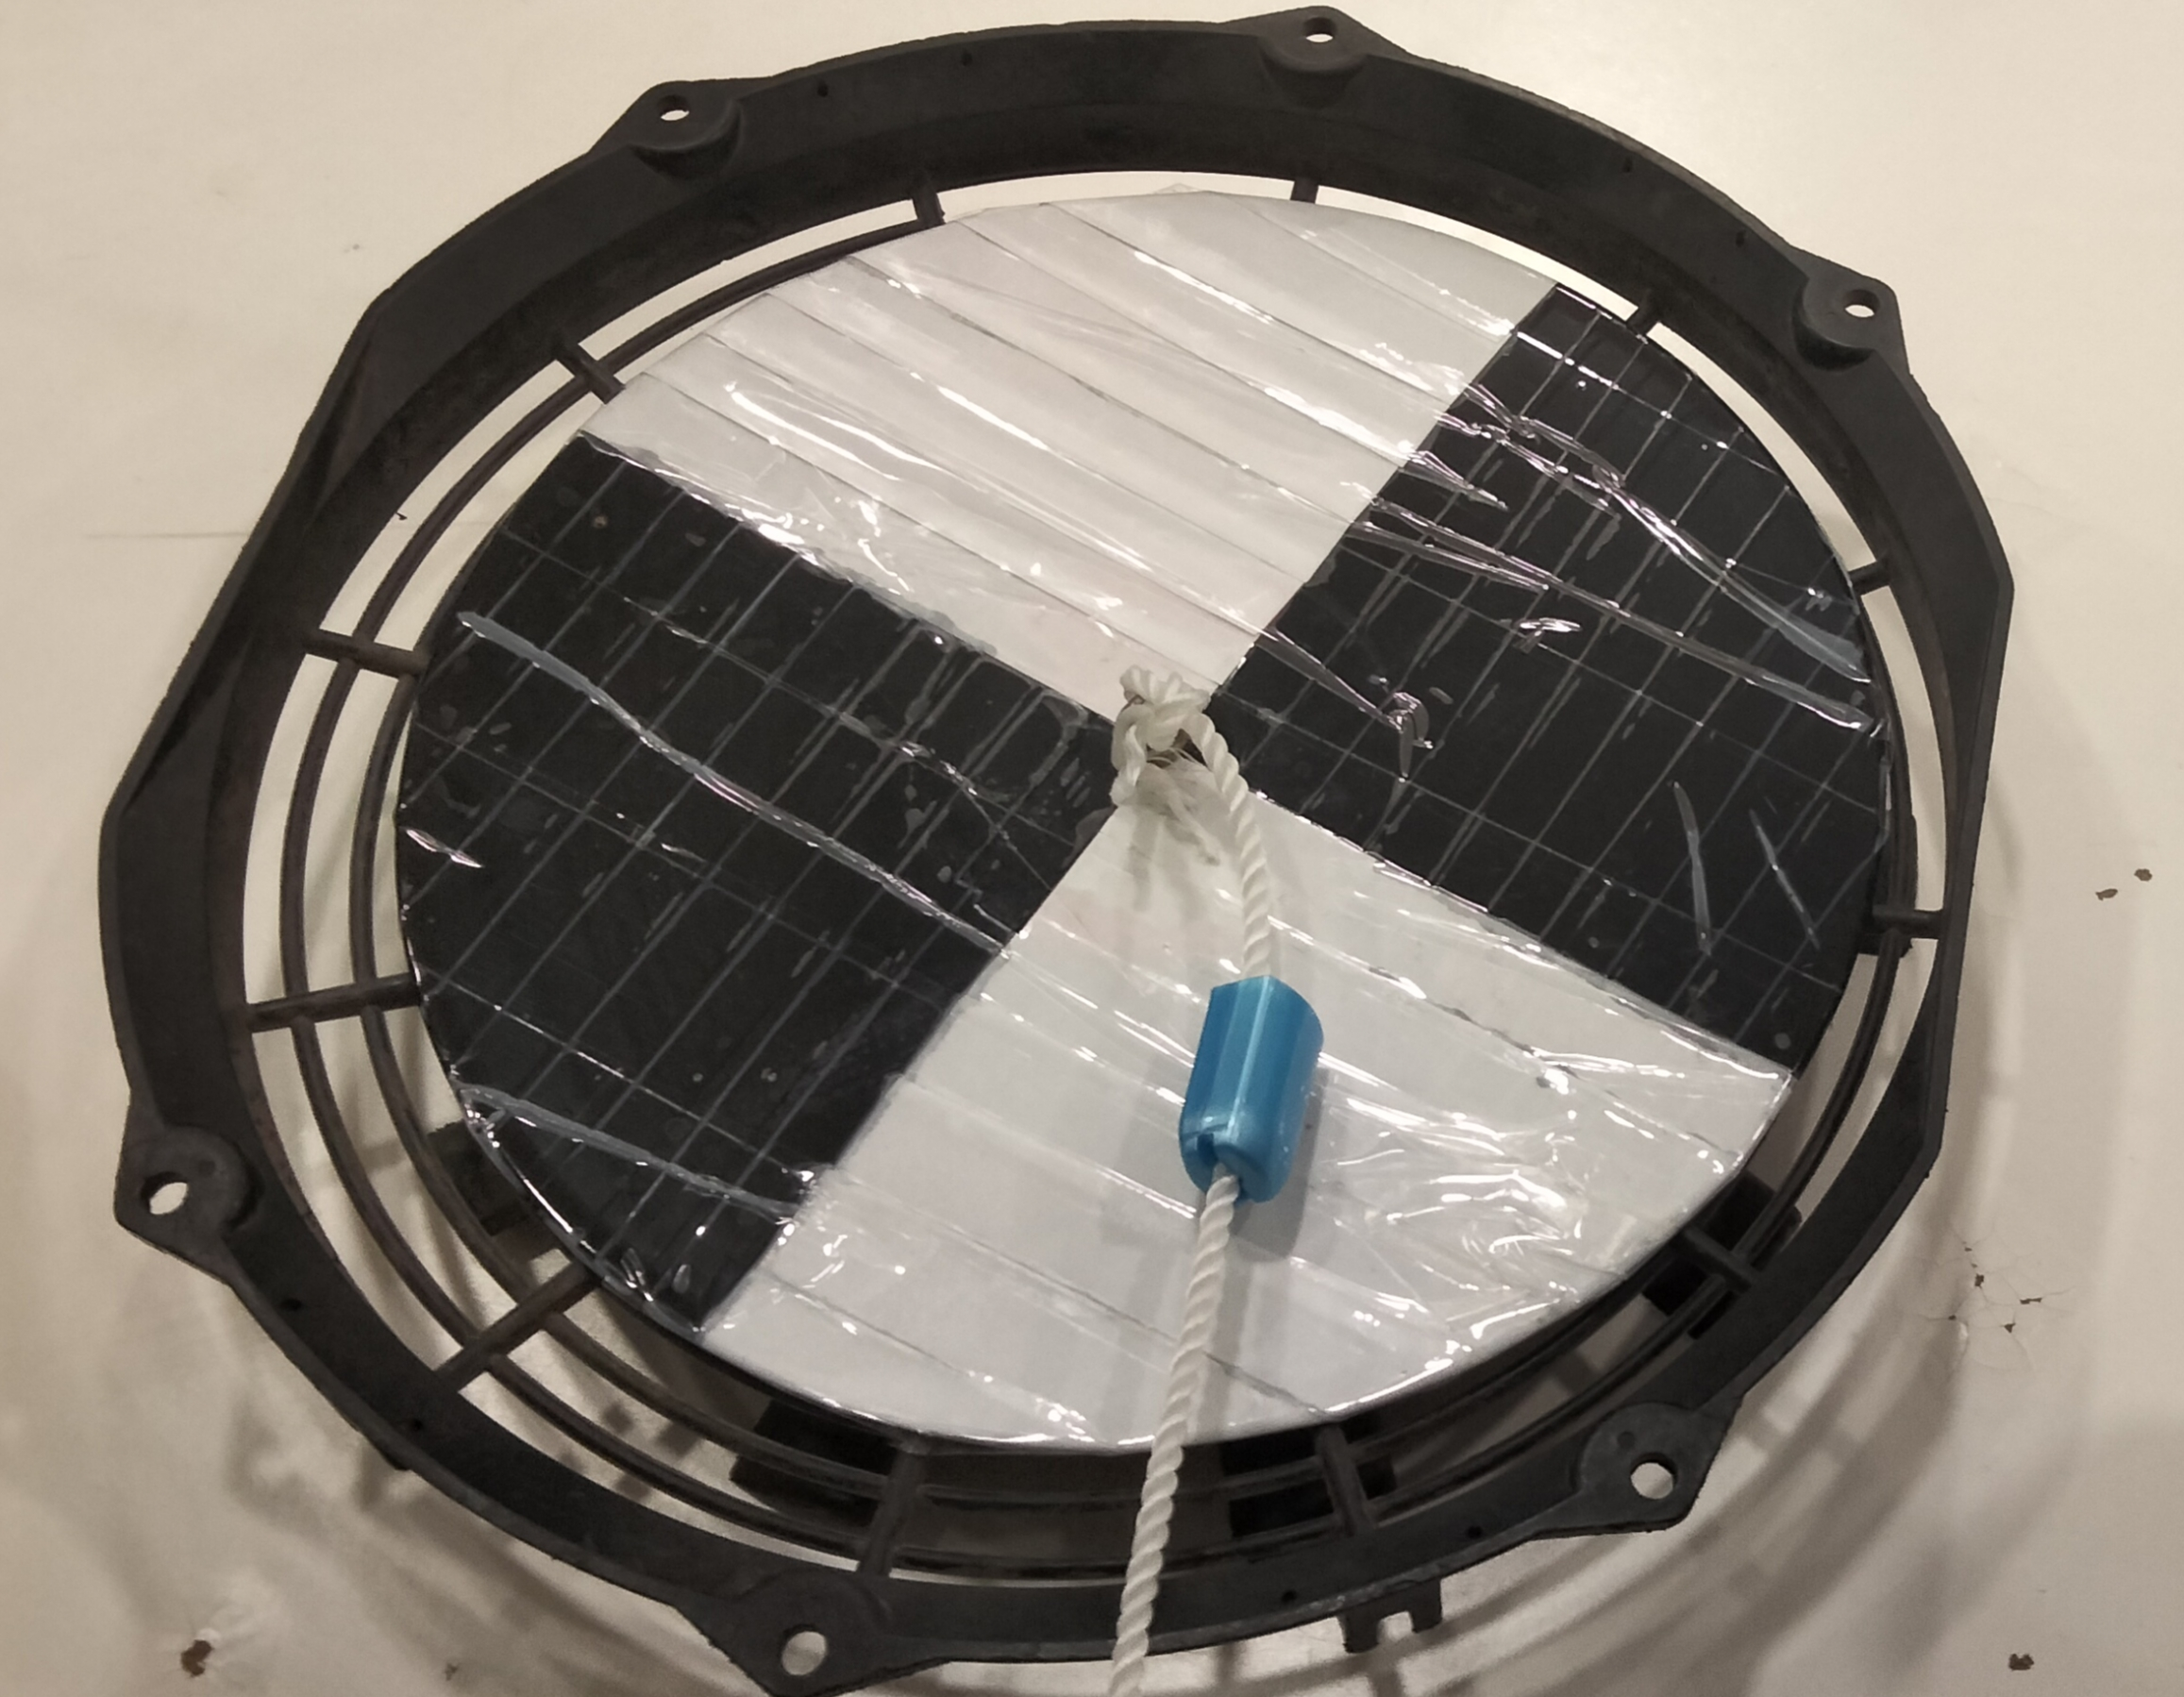
\includegraphics[scale=0.1]{070_design/package/55_disk.jpg}
\caption{\gls{DIY} Secchi Disk with weight added [own picture]}
\end{figure}